\documentclass[11pt]{article}
\usepackage[margin=1in]{geometry}
\usepackage{graphicx}
\usepackage{float}
\title{Project Deliverable 2}
\author{Group 4}
\date{}

\graphicspath{ {img/} }

\begin{document}
\maketitle

\subsection*{Introduction}

The group has performed initial research on three algorithms. One solves a clustering problem, one solves the Exact Cover problem, and one solves path planning with unreliable information.

\subsection*{Algorithm 1: K-Median}

$k$-Median is a cluster-analysis strategy to solve a cluster distance minimization problem. The problem is nearly identical to the $k$-Means problem. The difference is that in $k$-Means, the average points may be calculated, while in $k$-Median, the solution set must be a subset of the input. The goal is to minimize the distance from all points to their nearest median point.

A K-Medians instance is a tuple $(k,F,C,d)$, where k is the number of median points, $F$ is the set of solution candidates, $C$ is the set of all points, and $d(j,S)$ is the distance from point $j$ to the nearest point in $S$. The solution $H \in F$ is one in which Equation 1 is minimized [3].
$$\sum_{c \in C} d(c,H)$$
\begin{center}
    Equation 1
\end{center}

A proposed solution to this problem uses local search. Propose a solution $H \in F$ to begin with and calculate its score. Then, incrementally swap out points one at a time with the median points and score the result, tracking the best score and attempting to minimize that. The solution is not guaranteed to be optimal due to limitations in the local search technique. According to Pandit [4], the solution computed has an approximation ratio of 5, meaning that it is within five times the optimal solution.

\subsection*{Algorithm 2: Dancing Links}

Donald Knuth developed Dancing Links as an approach to implementing Algorithm X, which is a proposed solution to the Exact Cover problem [1]. The Exact Cover problem is described as follows:
$$Z_iZ, Z_i \subset Y$$
$$Y_jY, Y_j \notin Z_i$$

$Z^{\ast}$ is a solution to the exact cover problem if it satisfies the following constraints:
$$Z^{\ast} \subset Z$$
$$Z_{i}^{\ast} \cap Z_{j} = \emptyset $$
$$Z_{1}^{\ast} \cup Z_{2}^{\ast} \cup ... \cup Z_{n}^{\ast} = Y$$

A common way to represent the exact coverage problem is to let $Z$ be an $n$x$m$ matrix. The rows of this matrix represent $Z_i$ while the columns represent $Y_i$. If the set $Z_i$ contains the element $Y_j$ then $Z_{ij}=1$. Otherwise, $Z_{ij}=0$. The problem is to find some set of rows that have exactly one $1$ in each column, if such a solution exists.

Though other uses exist, Dancing Link's most apparent and direct use is to solve the Exact Cover problem. The matrix $Z$ is represented by a two-dimensional Linked List. Entries with value $0$ are not placed in the Linked List. In addition, each column has a header node that is used to traverse the matrix. The header nodes are connected to each other horizontally. Each node is connected horizontally to the closest $1$ in each of four directions (up, down, left, and right. The lists are circular, so the node to the right of the farthest right node of a row is the farthest left node of that row.

The algorithm is a recursive depth-first search with backtracking. With each recursion, a set of nodes is removed from the structure, terminating with the base case of an empty structure. The challenge lies in determining which nodes to remove. Knuth's solution is to choose an arbitrary column $i$, and choose a row $j$ where $Z_{ij}=1$. If such a row does not exist, there is no solution. Before returning, each row that has a $1$ in column $i$ is removed and each column that has a $1$ in row $j$ is removd. Row $j$ is included in the partial solution which will be returned by the recursive function.

\subsection*{Algorithm 3: D* Lite}

D* lite is a modern path planning algorithm proposed by Sven Koenig and Maxim Likhachev. Inspired by D*, D* Lite is actually a variation of Lifelong Planning A* (LPA*) with traits of D*, also made in part by Koenig. The motivation for D* Lite was to speed up path planning in unknown or dynamic maps. Classic path planning algorithms require recalculating the entirety of the path, or storing a great deal of information. Figure 1, taken from Koenig [4], demonstrates the replanning after a new obstacle is observed. Only the greyed cells have had their edge weights modified, as opposed to the entire map.

\begin{center}
    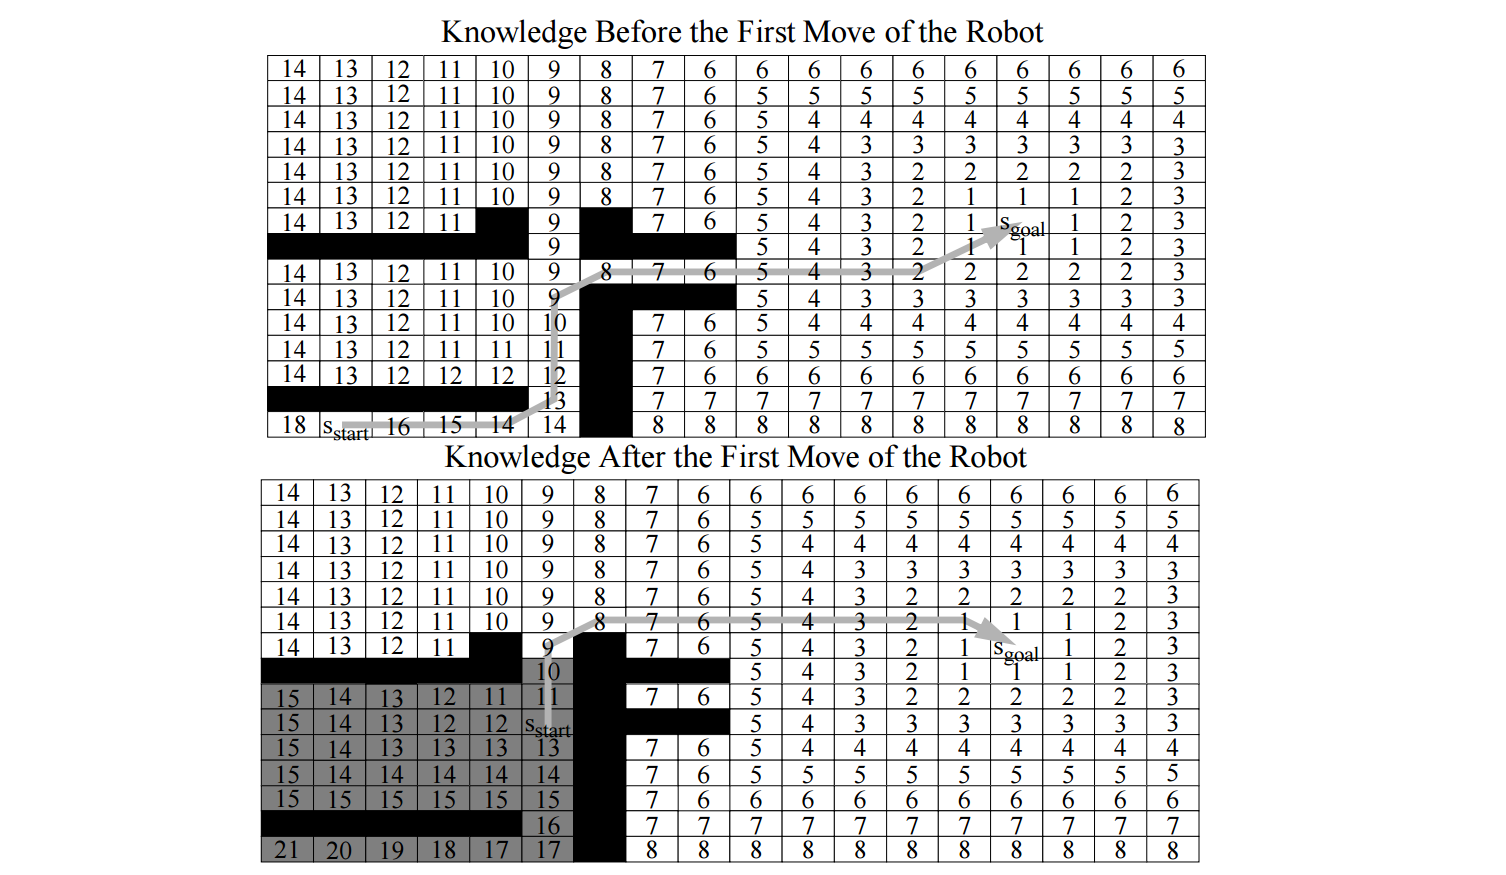
\includegraphics[scale=0.15]{dstarlite}
\end{center}

D* Lite functions by, upon encountering a previously unknown obstacle, propagating the changes in edge weights backwards and forwards as necessary. The main challenges come not from propagating these weights, but from doing so while maintaining as much of the previous, important, state as possible. This includes things like vertices in the priority queue whose edge weights have been altered. 

\section*{Works Cited}

[1] D. E. Knuth, ``Dancing Links'', Stanford University, November 15, 2000.\\\relax
[2] S. Koenig, M. Likhachev, ``D* Lite'', 2002.\\\relax
[3] S. Li, O. Svensson, ``Approximating k-Median via Pseudo-Approximation'', November 2, 2012.\\\relax
[4] V. Pandit, ``Local Search Based Approximation Algorithms: The k-median problem'', Bangalore, India, 2011.\\\relax

\end{document}
